\documentclass[twoside]{book}

% Packages required by doxygen
\usepackage{fixltx2e}
\usepackage{calc}
\usepackage{doxygen}
\usepackage[export]{adjustbox} % also loads graphicx
\usepackage{graphicx}
\usepackage[utf8]{inputenc}
\usepackage{makeidx}
\usepackage{multicol}
\usepackage{multirow}
\PassOptionsToPackage{warn}{textcomp}
\usepackage{textcomp}
\usepackage[nointegrals]{wasysym}
\usepackage[table]{xcolor}

% Font selection
\usepackage[T1]{fontenc}
\usepackage[scaled=.90]{helvet}
\usepackage{courier}
\usepackage{amssymb}
\usepackage{sectsty}
\renewcommand{\familydefault}{\sfdefault}
\allsectionsfont{%
  \fontseries{bc}\selectfont%
  \color{darkgray}%
}
\renewcommand{\DoxyLabelFont}{%
  \fontseries{bc}\selectfont%
  \color{darkgray}%
}
\newcommand{\+}{\discretionary{\mbox{\scriptsize$\hookleftarrow$}}{}{}}

% Page & text layout
\usepackage{geometry}
\geometry{%
  a4paper,%
  top=2.5cm,%
  bottom=2.5cm,%
  left=2.5cm,%
  right=2.5cm%
}
\tolerance=750
\hfuzz=15pt
\hbadness=750
\setlength{\emergencystretch}{15pt}
\setlength{\parindent}{0cm}
\setlength{\parskip}{3ex plus 2ex minus 2ex}
\makeatletter
\renewcommand{\paragraph}{%
  \@startsection{paragraph}{4}{0ex}{-1.0ex}{1.0ex}{%
    \normalfont\normalsize\bfseries\SS@parafont%
  }%
}
\renewcommand{\subparagraph}{%
  \@startsection{subparagraph}{5}{0ex}{-1.0ex}{1.0ex}{%
    \normalfont\normalsize\bfseries\SS@subparafont%
  }%
}
\makeatother

% Headers & footers
\usepackage{fancyhdr}
\pagestyle{fancyplain}
\fancyhead[LE]{\fancyplain{}{\bfseries\thepage}}
\fancyhead[CE]{\fancyplain{}{}}
\fancyhead[RE]{\fancyplain{}{\bfseries\leftmark}}
\fancyhead[LO]{\fancyplain{}{\bfseries\rightmark}}
\fancyhead[CO]{\fancyplain{}{}}
\fancyhead[RO]{\fancyplain{}{\bfseries\thepage}}
\fancyfoot[LE]{\fancyplain{}{}}
\fancyfoot[CE]{\fancyplain{}{}}
\fancyfoot[RE]{\fancyplain{}{\bfseries\scriptsize Generated by Doxygen }}
\fancyfoot[LO]{\fancyplain{}{\bfseries\scriptsize Generated by Doxygen }}
\fancyfoot[CO]{\fancyplain{}{}}
\fancyfoot[RO]{\fancyplain{}{}}
\renewcommand{\footrulewidth}{0.4pt}
\renewcommand{\chaptermark}[1]{%
  \markboth{#1}{}%
}
\renewcommand{\sectionmark}[1]{%
  \markright{\thesection\ #1}%
}

% Indices & bibliography
\usepackage{natbib}
\usepackage[titles]{tocloft}
\setcounter{tocdepth}{3}
\setcounter{secnumdepth}{5}
\makeindex

% Hyperlinks (required, but should be loaded last)
\usepackage{ifpdf}
\ifpdf
  \usepackage[pdftex,pagebackref=true]{hyperref}
\else
  \usepackage[ps2pdf,pagebackref=true]{hyperref}
\fi
\hypersetup{%
  colorlinks=true,%
  linkcolor=blue,%
  citecolor=blue,%
  unicode%
}

% Custom commands
\newcommand{\clearemptydoublepage}{%
  \newpage{\pagestyle{empty}\cleardoublepage}%
}

\usepackage{caption}
\captionsetup{labelsep=space,justification=centering,font={bf},singlelinecheck=off,skip=4pt,position=top}

%===== C O N T E N T S =====

\begin{document}

% Titlepage & ToC
\hypersetup{pageanchor=false,
             bookmarksnumbered=true,
             pdfencoding=unicode
            }
\pagenumbering{alph}
\begin{titlepage}
\vspace*{7cm}
\begin{center}%
{\Large My Project }\\
\vspace*{1cm}
{\large Generated by Doxygen 1.8.13}\\
\end{center}
\end{titlepage}
\clearemptydoublepage
\pagenumbering{roman}
\tableofcontents
\clearemptydoublepage
\pagenumbering{arabic}
\hypersetup{pageanchor=true}

%--- Begin generated contents ---
\chapter{Data Structure Index}
\section{Data Structures}
Here are the data structures with brief descriptions\+:\begin{DoxyCompactList}
\item\contentsline{section}{\hyperlink{struct_a_d_c_m_g_rcmd_info_type}{A\+D\+C\+M\+G\+Rcmd\+Info\+Type} }{\pageref{struct_a_d_c_m_g_rcmd_info_type}}{}
\item\contentsline{section}{\hyperlink{structcmd_queue__t}{cmd\+Queue\+\_\+t} }{\pageref{structcmd_queue__t}}{}
\item\contentsline{section}{\hyperlink{struct_timer_struct}{Timer\+Struct} }{\pageref{struct_timer_struct}}{}
\end{DoxyCompactList}

\chapter{File Index}
\section{File List}
Here is a list of all documented files with brief descriptions\+:\begin{DoxyCompactList}
\item\contentsline{section}{C\+:/\+Users/\+Karl/workspace\+\_\+v6\+\_\+2/\+L\+I\+L\+L\+E\+P\+O\+T\+T/\+H\+W/\hyperlink{_a_d_c_m_g_r_8c}{A\+D\+C\+M\+G\+R.\+c} \\*Documentation for A\+D\+C\+M\+GR module }{\pageref{_a_d_c_m_g_r_8c}}{}
\item\contentsline{section}{C\+:/\+Users/\+Karl/workspace\+\_\+v6\+\_\+2/\+L\+I\+L\+L\+E\+P\+O\+T\+T/\+H\+W/{\bfseries A\+D\+C\+M\+G\+R.\+h} }{\pageref{_a_d_c_m_g_r_8h}}{}
\item\contentsline{section}{C\+:/\+Users/\+Karl/workspace\+\_\+v6\+\_\+2/\+L\+I\+L\+L\+E\+P\+O\+T\+T/\+H\+W/\+L\+N\+K/\+Config/{\bfseries general.\+h} }{\pageref{general_8h}}{}
\item\contentsline{section}{C\+:/\+Users/\+Karl/workspace\+\_\+v6\+\_\+2/\+L\+I\+L\+L\+E\+P\+O\+T\+T/\+H\+W/\+L\+N\+K/\+Config/{\bfseries network.\+h} }{\pageref{network_8h}}{}
\item\contentsline{section}{C\+:/\+Users/\+Karl/workspace\+\_\+v6\+\_\+2/\+L\+I\+L\+L\+E\+P\+O\+T\+T/\+H\+W/\+L\+N\+K/\+Drivers/\hyperlink{gpio_8c}{gpio.\+c} }{\pageref{gpio_8c}}{}
\item\contentsline{section}{C\+:/\+Users/\+Karl/workspace\+\_\+v6\+\_\+2/\+L\+I\+L\+L\+E\+P\+O\+T\+T/\+H\+W/\+L\+N\+K/\+Drivers/{\bfseries gpio.\+h} }{\pageref{gpio_8h}}{}
\item\contentsline{section}{C\+:/\+Users/\+Karl/workspace\+\_\+v6\+\_\+2/\+L\+I\+L\+L\+E\+P\+O\+T\+T/\+H\+W/\+L\+N\+K/\+Drivers/{\bfseries mrf89xa.\+h} }{\pageref{mrf89xa_8h}}{}
\item\contentsline{section}{C\+:/\+Users/\+Karl/workspace\+\_\+v6\+\_\+2/\+L\+I\+L\+L\+E\+P\+O\+T\+T/\+H\+W/\+L\+N\+K/\+Drivers/{\bfseries system.\+h} }{\pageref{system_8h}}{}
\item\contentsline{section}{C\+:/\+Users/\+Karl/workspace\+\_\+v6\+\_\+2/\+L\+I\+L\+L\+E\+P\+O\+T\+T/\+H\+W/\+L\+N\+K/\+Drivers/\+Communication/{\bfseries spi.\+h} }{\pageref{spi_8h}}{}
\item\contentsline{section}{C\+:/\+Users/\+Karl/workspace\+\_\+v6\+\_\+2/\+L\+I\+L\+L\+E\+P\+O\+T\+T/\+H\+W/\+L\+N\+K/\+Drivers/\+Communication/{\bfseries uart.\+h} }{\pageref{uart_8h}}{}
\item\contentsline{section}{C\+:/\+Users/\+Karl/workspace\+\_\+v6\+\_\+2/\+L\+I\+L\+L\+E\+P\+O\+T\+T/\+H\+W/\+L\+N\+K/\+L\+N\+K/{\bfseries radio.\+h} }{\pageref{radio_8h}}{}
\item\contentsline{section}{C\+:/\+Users/\+Karl/workspace\+\_\+v6\+\_\+2/\+L\+I\+L\+L\+E\+P\+O\+T\+T/\+L\+O\+G\+I\+C/\hyperlink{application_8c}{application.\+c} }{\pageref{application_8c}}{}
\item\contentsline{section}{C\+:/\+Users/\+Karl/workspace\+\_\+v6\+\_\+2/\+L\+I\+L\+L\+E\+P\+O\+T\+T/\+L\+O\+G\+I\+C/{\bfseries application.\+h} }{\pageref{application_8h}}{}
\item\contentsline{section}{C\+:/\+Users/\+Karl/workspace\+\_\+v6\+\_\+2/\+L\+I\+L\+L\+E\+P\+O\+T\+T/\+M\+C\+U/\hyperlink{_a_d_c_8c}{A\+D\+C.\+c} \\*A\+DC hardware abstraction }{\pageref{_a_d_c_8c}}{}
\item\contentsline{section}{C\+:/\+Users/\+Karl/workspace\+\_\+v6\+\_\+2/\+L\+I\+L\+L\+E\+P\+O\+T\+T/\+M\+C\+U/{\bfseries A\+D\+C.\+h} }{\pageref{_a_d_c_8h}}{}
\item\contentsline{section}{C\+:/\+Users/\+Karl/workspace\+\_\+v6\+\_\+2/\+L\+I\+L\+L\+E\+P\+O\+T\+T/\+M\+C\+U/\hyperlink{clock_8c}{clock.\+c} }{\pageref{clock_8c}}{}
\item\contentsline{section}{C\+:/\+Users/\+Karl/workspace\+\_\+v6\+\_\+2/\+L\+I\+L\+L\+E\+P\+O\+T\+T/\+M\+C\+U/{\bfseries clock.\+h} }{\pageref{clock_8h}}{}
\item\contentsline{section}{C\+:/\+Users/\+Karl/workspace\+\_\+v6\+\_\+2/\+L\+I\+L\+L\+E\+P\+O\+T\+T/\+M\+C\+U/\hyperlink{misc_8c}{misc.\+c} }{\pageref{misc_8c}}{}
\item\contentsline{section}{C\+:/\+Users/\+Karl/workspace\+\_\+v6\+\_\+2/\+L\+I\+L\+L\+E\+P\+O\+T\+T/\+M\+C\+U/{\bfseries misc.\+h} }{\pageref{misc_8h}}{}
\item\contentsline{section}{C\+:/\+Users/\+Karl/workspace\+\_\+v6\+\_\+2/\+L\+I\+L\+L\+E\+P\+O\+T\+T/\+M\+C\+U/{\bfseries timer.\+h} }{\pageref{timer_8h}}{}
\item\contentsline{section}{C\+:/\+Users/\+Karl/workspace\+\_\+v6\+\_\+2/\+L\+I\+L\+L\+E\+P\+O\+T\+T/\+M\+C\+U/\hyperlink{wdt_8c}{wdt.\+c} \\*Documentation for the watchdog module }{\pageref{wdt_8c}}{}
\item\contentsline{section}{C\+:/\+Users/\+Karl/workspace\+\_\+v6\+\_\+2/\+L\+I\+L\+L\+E\+P\+O\+T\+T/\+M\+C\+U/{\bfseries wdt.\+h} }{\pageref{wdt_8h}}{}
\end{DoxyCompactList}

\chapter{Data Structure Documentation}
\hypertarget{struct_a_d_c_m_g_rcmd_info_type}{}\section{A\+D\+C\+M\+G\+Rcmd\+Info\+Type Struct Reference}
\label{struct_a_d_c_m_g_rcmd_info_type}\index{A\+D\+C\+M\+G\+Rcmd\+Info\+Type@{A\+D\+C\+M\+G\+Rcmd\+Info\+Type}}
\subsection*{Data Fields}
\begin{DoxyCompactItemize}
\item 
\mbox{\Hypertarget{struct_a_d_c_m_g_rcmd_info_type_a18b5981baee94493a2bd06ff64a87918}\label{struct_a_d_c_m_g_rcmd_info_type_a18b5981baee94493a2bd06ff64a87918}} 
uint8 {\bfseries sample\+\_\+size}
\item 
\mbox{\Hypertarget{struct_a_d_c_m_g_rcmd_info_type_a3f78b0ce54a6f57f456bf97022424d19}\label{struct_a_d_c_m_g_rcmd_info_type_a3f78b0ce54a6f57f456bf97022424d19}} 
A\+D\+C\+\_\+conf\+Type {\bfseries A\+D\+C\+\_\+configuration}
\end{DoxyCompactItemize}


The documentation for this struct was generated from the following file\+:\begin{DoxyCompactItemize}
\item 
C\+:/\+Users/\+Karl/workspace\+\_\+v6\+\_\+2/\+L\+I\+L\+L\+E\+P\+O\+T\+T/\+H\+W/A\+D\+C\+M\+G\+R.\+h\end{DoxyCompactItemize}

\hypertarget{structcmd_queue__t}{}\section{cmd\+Queue\+\_\+t Struct Reference}
\label{structcmd_queue__t}\index{cmd\+Queue\+\_\+t@{cmd\+Queue\+\_\+t}}
\subsection*{Data Fields}
\begin{DoxyCompactItemize}
\item 
\mbox{\Hypertarget{structcmd_queue__t_ab0c685bdd8ab7b18cb56c909e479bf6e}\label{structcmd_queue__t_ab0c685bdd8ab7b18cb56c909e479bf6e}} 
command\+Type $\ast$ {\bfseries commands}
\item 
\mbox{\Hypertarget{structcmd_queue__t_afd7e07fd89d37728eaa1d5300e4c73e9}\label{structcmd_queue__t_afd7e07fd89d37728eaa1d5300e4c73e9}} 
uint8 {\bfseries head}
\item 
\mbox{\Hypertarget{structcmd_queue__t_a5364ea4ecf1fd8513425b21373d152cc}\label{structcmd_queue__t_a5364ea4ecf1fd8513425b21373d152cc}} 
uint8 {\bfseries tail}
\item 
\mbox{\Hypertarget{structcmd_queue__t_abf7f47b9039221e81ecb5eac8f3b090d}\label{structcmd_queue__t_abf7f47b9039221e81ecb5eac8f3b090d}} 
uint8 {\bfseries size}
\end{DoxyCompactItemize}


The documentation for this struct was generated from the following file\+:\begin{DoxyCompactItemize}
\item 
C\+:/\+Users/\+Karl/workspace\+\_\+v6\+\_\+2/\+L\+I\+L\+L\+E\+P\+O\+T\+T/\+H\+W/A\+D\+C\+M\+G\+R.\+h\end{DoxyCompactItemize}

\hypertarget{struct_timer_struct}{}\section{Timer\+Struct Struct Reference}
\label{struct_timer_struct}\index{Timer\+Struct@{Timer\+Struct}}
\subsection*{Data Fields}
\begin{DoxyCompactItemize}
\item 
\mbox{\Hypertarget{struct_timer_struct_a30f756807d48ebf4e3821e88a072f327}\label{struct_timer_struct_a30f756807d48ebf4e3821e88a072f327}} 
unsigned long long int {\bfseries start\+Time}
\item 
\mbox{\Hypertarget{struct_timer_struct_a583e600345545436751b8cc665bef6aa}\label{struct_timer_struct_a583e600345545436751b8cc665bef6aa}} 
unsigned long long int {\bfseries end\+Time}
\item 
\mbox{\Hypertarget{struct_timer_struct_a6b18ee2f4d766334e881f585523ce7e9}\label{struct_timer_struct_a6b18ee2f4d766334e881f585523ce7e9}} 
unsigned long long int {\bfseries elapsed}
\end{DoxyCompactItemize}


The documentation for this struct was generated from the following file\+:\begin{DoxyCompactItemize}
\item 
C\+:/\+Users/\+Karl/workspace\+\_\+v6\+\_\+2/\+L\+I\+L\+L\+E\+P\+O\+T\+T/\+M\+C\+U/timer.\+h\end{DoxyCompactItemize}

\chapter{File Documentation}
\hypertarget{_a_d_c_m_g_r_8c}{}\section{C\+:/\+Users/\+Karl/workspace\+\_\+v6\+\_\+2/\+L\+I\+L\+L\+E\+P\+O\+T\+T/\+H\+W/\+A\+D\+C\+M\+GR.c File Reference}
\label{_a_d_c_m_g_r_8c}\index{C\+:/\+Users/\+Karl/workspace\+\_\+v6\+\_\+2/\+L\+I\+L\+L\+E\+P\+O\+T\+T/\+H\+W/\+A\+D\+C\+M\+G\+R.\+c@{C\+:/\+Users/\+Karl/workspace\+\_\+v6\+\_\+2/\+L\+I\+L\+L\+E\+P\+O\+T\+T/\+H\+W/\+A\+D\+C\+M\+G\+R.\+c}}


Documentation for A\+D\+C\+M\+GR module.  


{\ttfamily \#include \char`\"{}A\+D\+C\+M\+G\+R.\+h\char`\"{}}\newline
Include dependency graph for A\+D\+C\+M\+G\+R.\+c\+:\nopagebreak
\begin{figure}[H]
\begin{center}
\leavevmode
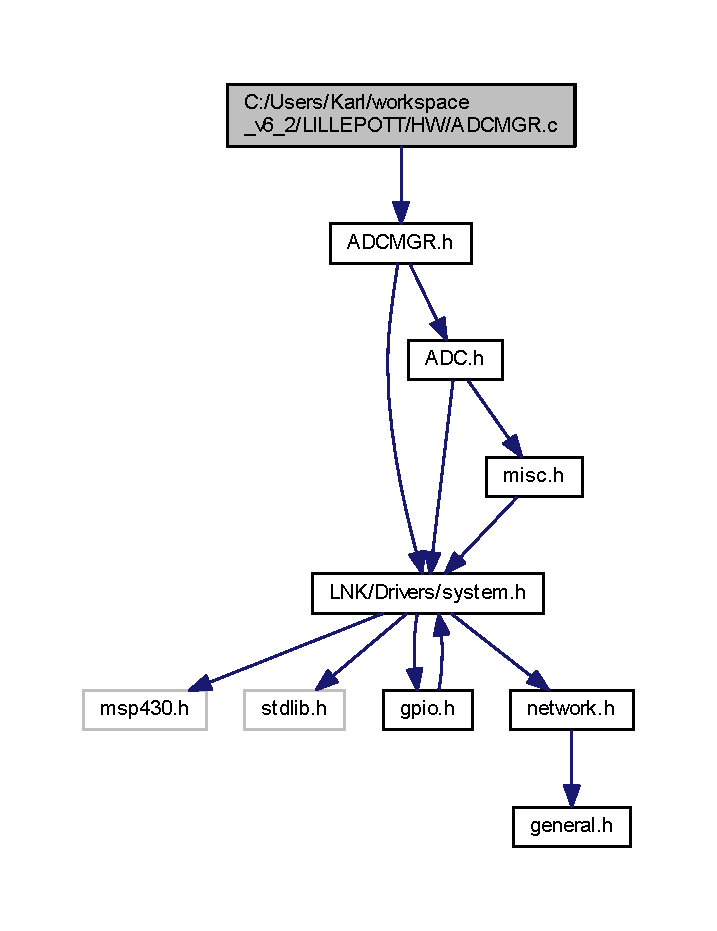
\includegraphics[width=344pt]{_a_d_c_m_g_r_8c__incl}
\end{center}
\end{figure}
\subsection*{Macros}
\begin{DoxyCompactItemize}
\item 
\#define \hyperlink{_a_d_c_m_g_r_8c_af3f1f095c6a3e15fb326180be23523e5}{A\+D\+C\+M\+G\+R\+\_\+\+C\+O\+M\+M\+A\+N\+D\+\_\+\+B\+U\+F\+F\+E\+R\+\_\+\+S\+I\+ZE}~(sizeof(buf) / sizeof(command\+Type))
\item 
\#define \hyperlink{_a_d_c_m_g_r_8c_a586e570c38cfcbc5c9ba0efe9abd605f}{C\+O\+M\+M\+A\+N\+D\+S\+\_\+\+A\+R\+R\+A\+Y\+\_\+\+S\+I\+ZE}~sizeof(priv\+\_\+commands) / sizeof(\hyperlink{struct_a_d_c_m_g_rcmd_info_type}{A\+D\+C\+M\+G\+Rcmd\+Info\+Type})
\end{DoxyCompactItemize}
\subsection*{Functions}
\begin{DoxyCompactItemize}
\item 
\mbox{\Hypertarget{_a_d_c_m_g_r_8c_af2bce5b4131a4bf18bc45656be658194}\label{_a_d_c_m_g_r_8c_af2bce5b4131a4bf18bc45656be658194}} 
void {\bfseries init\+Cmd\+Queue} (\hyperlink{structcmd_queue__t}{cmd\+Queue\+\_\+t} $\ast$f, uint8 size)
\item 
\mbox{\Hypertarget{_a_d_c_m_g_r_8c_a3d43487506ff4ee2ea6231eb6346d75b}\label{_a_d_c_m_g_r_8c_a3d43487506ff4ee2ea6231eb6346d75b}} 
command\+Type {\bfseries read\+Cmd\+From\+Queue} (\hyperlink{structcmd_queue__t}{cmd\+Queue\+\_\+t} $\ast$f)
\item 
\mbox{\Hypertarget{_a_d_c_m_g_r_8c_abea7e84cb7a59993cbea2e6cd5d82c88}\label{_a_d_c_m_g_r_8c_abea7e84cb7a59993cbea2e6cd5d82c88}} 
uint16 {\bfseries A\+D\+C\+M\+G\+R\+\_\+get\+Temp} ()
\item 
\mbox{\Hypertarget{_a_d_c_m_g_r_8c_a1ba925b1b204c109c7904158bab95818}\label{_a_d_c_m_g_r_8c_a1ba925b1b204c109c7904158bab95818}} 
uint16 {\bfseries A\+D\+C\+M\+G\+R\+\_\+get\+Hum} ()
\item 
\mbox{\Hypertarget{_a_d_c_m_g_r_8c_a22264ef7773c4954a850765930385e62}\label{_a_d_c_m_g_r_8c_a22264ef7773c4954a850765930385e62}} 
uint16 {\bfseries A\+D\+C\+M\+G\+R\+\_\+get\+Battery} ()
\item 
\mbox{\Hypertarget{_a_d_c_m_g_r_8c_a603cd40c54c178b5fb6c5fe36b509dd7}\label{_a_d_c_m_g_r_8c_a603cd40c54c178b5fb6c5fe36b509dd7}} 
\hyperlink{structcmd_queue__t}{cmd\+Queue\+\_\+t} $\ast$ {\bfseries A\+D\+C\+M\+G\+R\+\_\+get\+Cmd\+Queue} ()
\item 
\mbox{\Hypertarget{_a_d_c_m_g_r_8c_a4a075ee42393672a6d8fdbe1047f9805}\label{_a_d_c_m_g_r_8c_a4a075ee42393672a6d8fdbe1047f9805}} 
A\+D\+C\+M\+G\+R\+\_\+state {\bfseries A\+D\+C\+M\+G\+R\+\_\+get\+State} ()
\item 
\mbox{\Hypertarget{_a_d_c_m_g_r_8c_a97052a601114641d3ec6fbe67c17ef6e}\label{_a_d_c_m_g_r_8c_a97052a601114641d3ec6fbe67c17ef6e}} 
void {\bfseries A\+D\+C\+M\+G\+R\+\_\+set\+State} (A\+D\+C\+M\+G\+R\+\_\+state state)
\item 
\mbox{\Hypertarget{_a_d_c_m_g_r_8c_a7fbb04a15eced23de9df7e0bbe0f8ed3}\label{_a_d_c_m_g_r_8c_a7fbb04a15eced23de9df7e0bbe0f8ed3}} 
command\+Type {\bfseries A\+D\+C\+M\+G\+R\+\_\+get\+Cmd} ()
\item 
\mbox{\Hypertarget{_a_d_c_m_g_r_8c_a1b48639426304025fbdfd1285f7e7195}\label{_a_d_c_m_g_r_8c_a1b48639426304025fbdfd1285f7e7195}} 
void {\bfseries A\+D\+C\+M\+G\+R\+\_\+set\+Cmd} (command\+Type cmd)
\item 
\mbox{\Hypertarget{_a_d_c_m_g_r_8c_a061b3949a44b11940952d1d78fb1266f}\label{_a_d_c_m_g_r_8c_a061b3949a44b11940952d1d78fb1266f}} 
uint8 {\bfseries A\+D\+C\+M\+G\+R\+\_\+add\+Cmd\+To\+Queue} (\hyperlink{structcmd_queue__t}{cmd\+Queue\+\_\+t} $\ast$f, command\+Type command)
\item 
\mbox{\Hypertarget{_a_d_c_m_g_r_8c_ad72756943539c04e7f2224b0667ed7db}\label{_a_d_c_m_g_r_8c_ad72756943539c04e7f2224b0667ed7db}} 
void {\bfseries A\+D\+C\+M\+G\+R\+\_\+init} ()
\item 
\mbox{\Hypertarget{_a_d_c_m_g_r_8c_a4e020603caacdd6bb75bebf030cc06fa}\label{_a_d_c_m_g_r_8c_a4e020603caacdd6bb75bebf030cc06fa}} 
void {\bfseries A\+D\+C\+M\+G\+R\+\_\+cyclic} ()
\end{DoxyCompactItemize}
\subsection*{Variables}
\begin{DoxyCompactItemize}
\item 
const \hyperlink{struct_a_d_c_m_g_rcmd_info_type}{A\+D\+C\+M\+G\+Rcmd\+Info\+Type} {\bfseries priv\+\_\+commands} \mbox{[}$\,$\mbox{]}
\end{DoxyCompactItemize}


\subsection{Detailed Description}
Documentation for A\+D\+C\+M\+GR module. 


\begin{DoxyImageNoCaption}
  \mbox{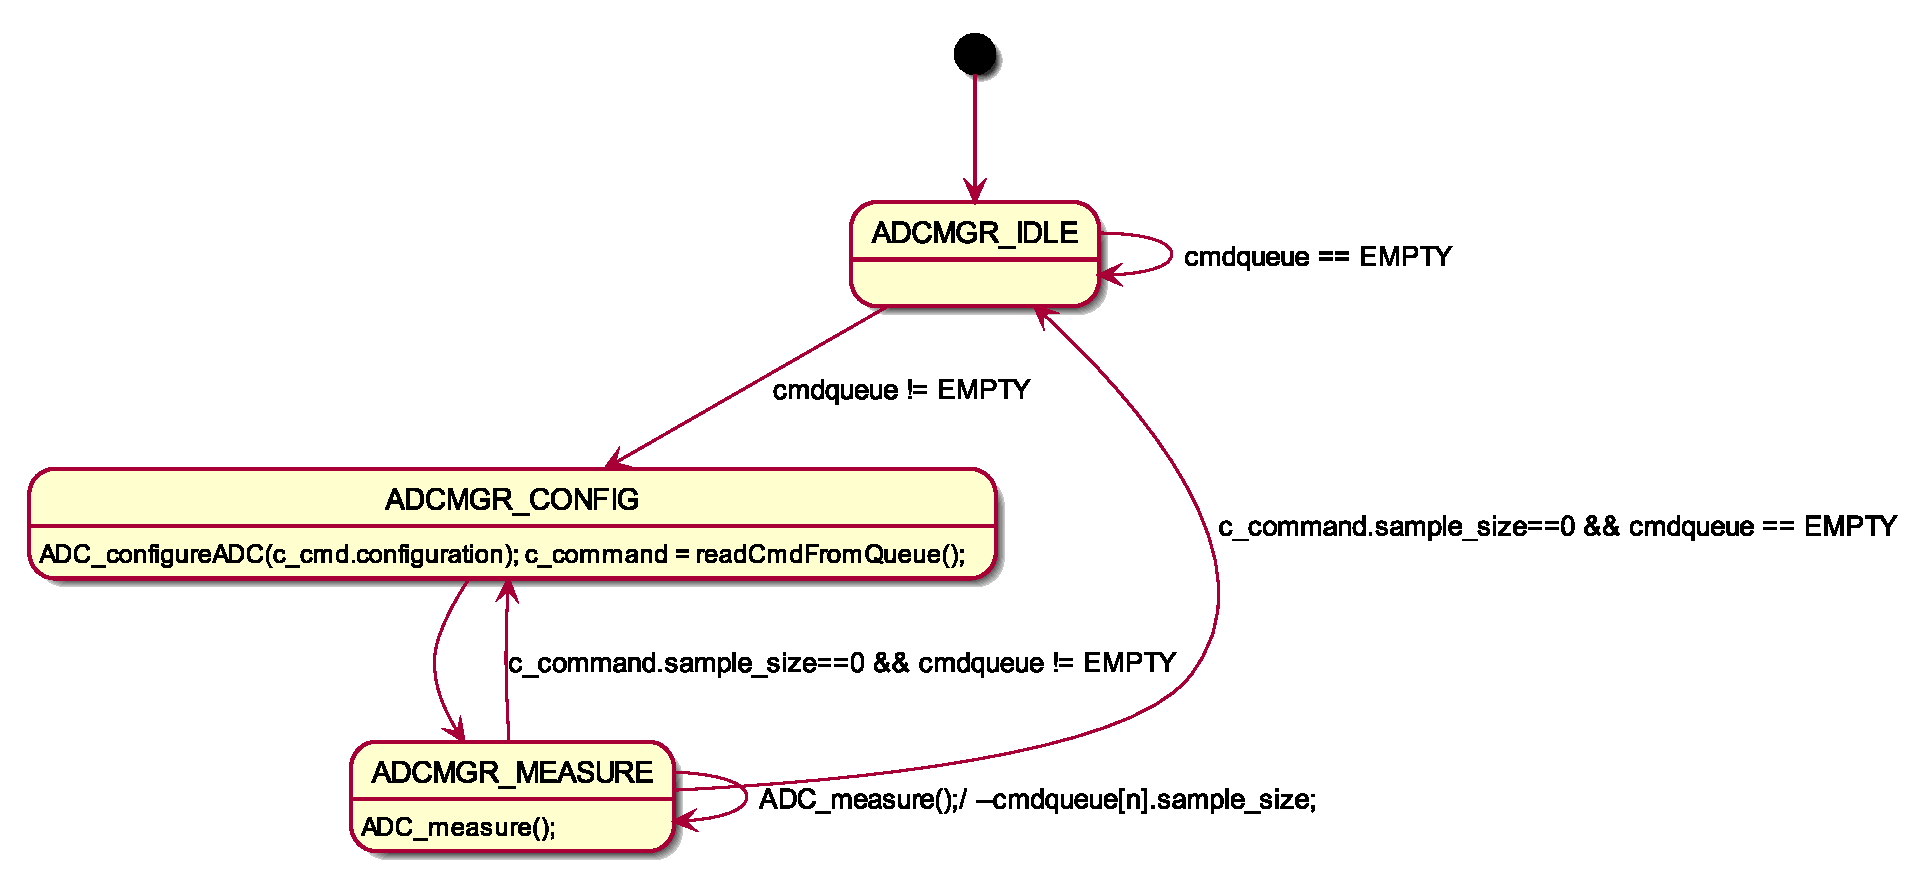
\includegraphics[width=\textwidth,height=\textheight/2,keepaspectratio=true]{ADCMGR_STATECHART}}
\end{DoxyImageNoCaption}
 

\subsection{Macro Definition Documentation}
\mbox{\Hypertarget{_a_d_c_m_g_r_8c_af3f1f095c6a3e15fb326180be23523e5}\label{_a_d_c_m_g_r_8c_af3f1f095c6a3e15fb326180be23523e5}} 
\index{A\+D\+C\+M\+G\+R.\+c@{A\+D\+C\+M\+G\+R.\+c}!A\+D\+C\+M\+G\+R\+\_\+\+C\+O\+M\+M\+A\+N\+D\+\_\+\+B\+U\+F\+F\+E\+R\+\_\+\+S\+I\+ZE@{A\+D\+C\+M\+G\+R\+\_\+\+C\+O\+M\+M\+A\+N\+D\+\_\+\+B\+U\+F\+F\+E\+R\+\_\+\+S\+I\+ZE}}
\index{A\+D\+C\+M\+G\+R\+\_\+\+C\+O\+M\+M\+A\+N\+D\+\_\+\+B\+U\+F\+F\+E\+R\+\_\+\+S\+I\+ZE@{A\+D\+C\+M\+G\+R\+\_\+\+C\+O\+M\+M\+A\+N\+D\+\_\+\+B\+U\+F\+F\+E\+R\+\_\+\+S\+I\+ZE}!A\+D\+C\+M\+G\+R.\+c@{A\+D\+C\+M\+G\+R.\+c}}
\subsubsection{\texorpdfstring{A\+D\+C\+M\+G\+R\+\_\+\+C\+O\+M\+M\+A\+N\+D\+\_\+\+B\+U\+F\+F\+E\+R\+\_\+\+S\+I\+ZE}{ADCMGR\_COMMAND\_BUFFER\_SIZE}}
{\footnotesize\ttfamily \#define A\+D\+C\+M\+G\+R\+\_\+\+C\+O\+M\+M\+A\+N\+D\+\_\+\+B\+U\+F\+F\+E\+R\+\_\+\+S\+I\+ZE~(sizeof(buf) / sizeof(command\+Type))}

command buffer size \mbox{\Hypertarget{_a_d_c_m_g_r_8c_a586e570c38cfcbc5c9ba0efe9abd605f}\label{_a_d_c_m_g_r_8c_a586e570c38cfcbc5c9ba0efe9abd605f}} 
\index{A\+D\+C\+M\+G\+R.\+c@{A\+D\+C\+M\+G\+R.\+c}!C\+O\+M\+M\+A\+N\+D\+S\+\_\+\+A\+R\+R\+A\+Y\+\_\+\+S\+I\+ZE@{C\+O\+M\+M\+A\+N\+D\+S\+\_\+\+A\+R\+R\+A\+Y\+\_\+\+S\+I\+ZE}}
\index{C\+O\+M\+M\+A\+N\+D\+S\+\_\+\+A\+R\+R\+A\+Y\+\_\+\+S\+I\+ZE@{C\+O\+M\+M\+A\+N\+D\+S\+\_\+\+A\+R\+R\+A\+Y\+\_\+\+S\+I\+ZE}!A\+D\+C\+M\+G\+R.\+c@{A\+D\+C\+M\+G\+R.\+c}}
\subsubsection{\texorpdfstring{C\+O\+M\+M\+A\+N\+D\+S\+\_\+\+A\+R\+R\+A\+Y\+\_\+\+S\+I\+ZE}{COMMANDS\_ARRAY\_SIZE}}
{\footnotesize\ttfamily \#define C\+O\+M\+M\+A\+N\+D\+S\+\_\+\+A\+R\+R\+A\+Y\+\_\+\+S\+I\+ZE~sizeof(priv\+\_\+commands) / sizeof(\hyperlink{struct_a_d_c_m_g_rcmd_info_type}{A\+D\+C\+M\+G\+Rcmd\+Info\+Type})}

number of commands for A\+D\+C\+M\+GR 

\subsection{Variable Documentation}
\mbox{\Hypertarget{_a_d_c_m_g_r_8c_a1d455a591f2ca8a5ec256ba4841fd82e}\label{_a_d_c_m_g_r_8c_a1d455a591f2ca8a5ec256ba4841fd82e}} 
\index{A\+D\+C\+M\+G\+R.\+c@{A\+D\+C\+M\+G\+R.\+c}!priv\+\_\+commands@{priv\+\_\+commands}}
\index{priv\+\_\+commands@{priv\+\_\+commands}!A\+D\+C\+M\+G\+R.\+c@{A\+D\+C\+M\+G\+R.\+c}}
\subsubsection{\texorpdfstring{priv\+\_\+commands}{priv\_commands}}
{\footnotesize\ttfamily const \hyperlink{struct_a_d_c_m_g_rcmd_info_type}{A\+D\+C\+M\+G\+Rcmd\+Info\+Type} priv\+\_\+commands\mbox{[}$\,$\mbox{]}}

{\bfseries Initial value\+:}
\begin{DoxyCode}
=
\{

  
    \{    0,     ADC\_IDLE\},
    \{    1,     ADC\_TEMP\},
  \{    1,       ADC\_HUMIDITY\},
  \{    1,       ADC\_BATTERY\},

\}
\end{DoxyCode}

\hypertarget{gpio_8c}{}\section{C\+:/\+Users/\+Karl/workspace\+\_\+v6\+\_\+2/\+L\+I\+L\+L\+E\+P\+O\+T\+T/\+H\+W/\+L\+N\+K/\+Drivers/gpio.c File Reference}
\label{gpio_8c}\index{C\+:/\+Users/\+Karl/workspace\+\_\+v6\+\_\+2/\+L\+I\+L\+L\+E\+P\+O\+T\+T/\+H\+W/\+L\+N\+K/\+Drivers/gpio.\+c@{C\+:/\+Users/\+Karl/workspace\+\_\+v6\+\_\+2/\+L\+I\+L\+L\+E\+P\+O\+T\+T/\+H\+W/\+L\+N\+K/\+Drivers/gpio.\+c}}
{\ttfamily \#include \char`\"{}gpio.\+h\char`\"{}}\newline
Include dependency graph for gpio.\+c\+:\nopagebreak
\begin{figure}[H]
\begin{center}
\leavevmode
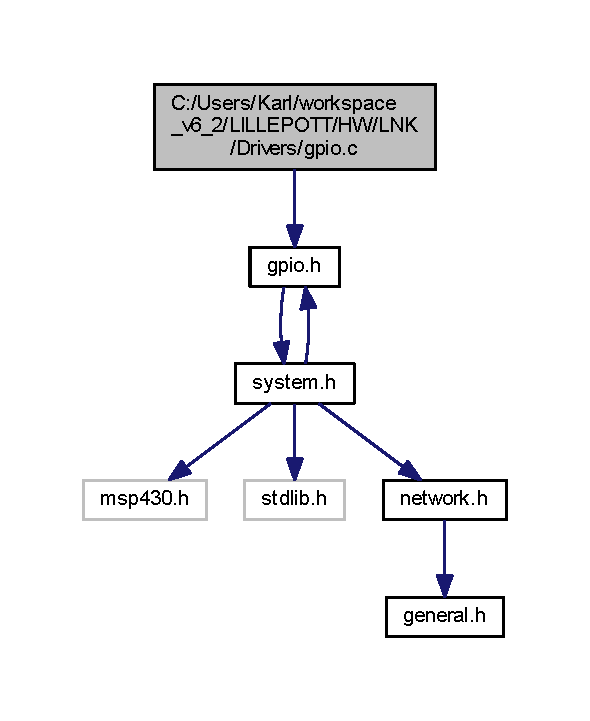
\includegraphics[width=283pt]{gpio_8c__incl}
\end{center}
\end{figure}
\subsection*{Functions}
\begin{DoxyCompactItemize}
\item 
void \hyperlink{gpio_8c_afc553591a466c3f20dce78f9cb80fab3}{G\+P\+I\+O\+\_\+setup} ()
\end{DoxyCompactItemize}


\subsection{Function Documentation}
\mbox{\Hypertarget{gpio_8c_afc553591a466c3f20dce78f9cb80fab3}\label{gpio_8c_afc553591a466c3f20dce78f9cb80fab3}} 
\index{gpio.\+c@{gpio.\+c}!G\+P\+I\+O\+\_\+setup@{G\+P\+I\+O\+\_\+setup}}
\index{G\+P\+I\+O\+\_\+setup@{G\+P\+I\+O\+\_\+setup}!gpio.\+c@{gpio.\+c}}
\subsubsection{\texorpdfstring{G\+P\+I\+O\+\_\+setup()}{GPIO\_setup()}}
{\footnotesize\ttfamily void G\+P\+I\+O\+\_\+setup (\begin{DoxyParamCaption}{ }\end{DoxyParamCaption})}

Configuring pins for minimal current consumption, for more info see family guide section 8.\+2.\+8 Used by RF module\+: P1.\+3 -\/ P1.\+7, P2.\+0-\/\+P2.\+1, P2.\+5 Unused\+: P1.\+0, P2.\+2-\/\+P2.\+4, P2.\+6-\/\+P2.\+7 
\hypertarget{application_8c}{}\section{C\+:/\+Users/\+Karl/workspace\+\_\+v6\+\_\+2/\+L\+I\+L\+L\+E\+P\+O\+T\+T/\+L\+O\+G\+I\+C/application.c File Reference}
\label{application_8c}\index{C\+:/\+Users/\+Karl/workspace\+\_\+v6\+\_\+2/\+L\+I\+L\+L\+E\+P\+O\+T\+T/\+L\+O\+G\+I\+C/application.\+c@{C\+:/\+Users/\+Karl/workspace\+\_\+v6\+\_\+2/\+L\+I\+L\+L\+E\+P\+O\+T\+T/\+L\+O\+G\+I\+C/application.\+c}}
{\ttfamily \#include $<$wdt.\+h$>$}\newline
{\ttfamily \#include \char`\"{}application.\+h\char`\"{}}\newline
{\ttfamily \#include \char`\"{}A\+D\+C\+M\+G\+R.\+h\char`\"{}}\newline
{\ttfamily \#include \char`\"{}network.\+h\char`\"{}}\newline
{\ttfamily \#include \char`\"{}general.\+h\char`\"{}}\newline
{\ttfamily \#include \char`\"{}uart.\+h\char`\"{}}\newline
{\ttfamily \#include \char`\"{}spi.\+h\char`\"{}}\newline
{\ttfamily \#include \char`\"{}radio.\+h\char`\"{}}\newline
Include dependency graph for application.\+c\+:\nopagebreak
\begin{figure}[H]
\begin{center}
\leavevmode
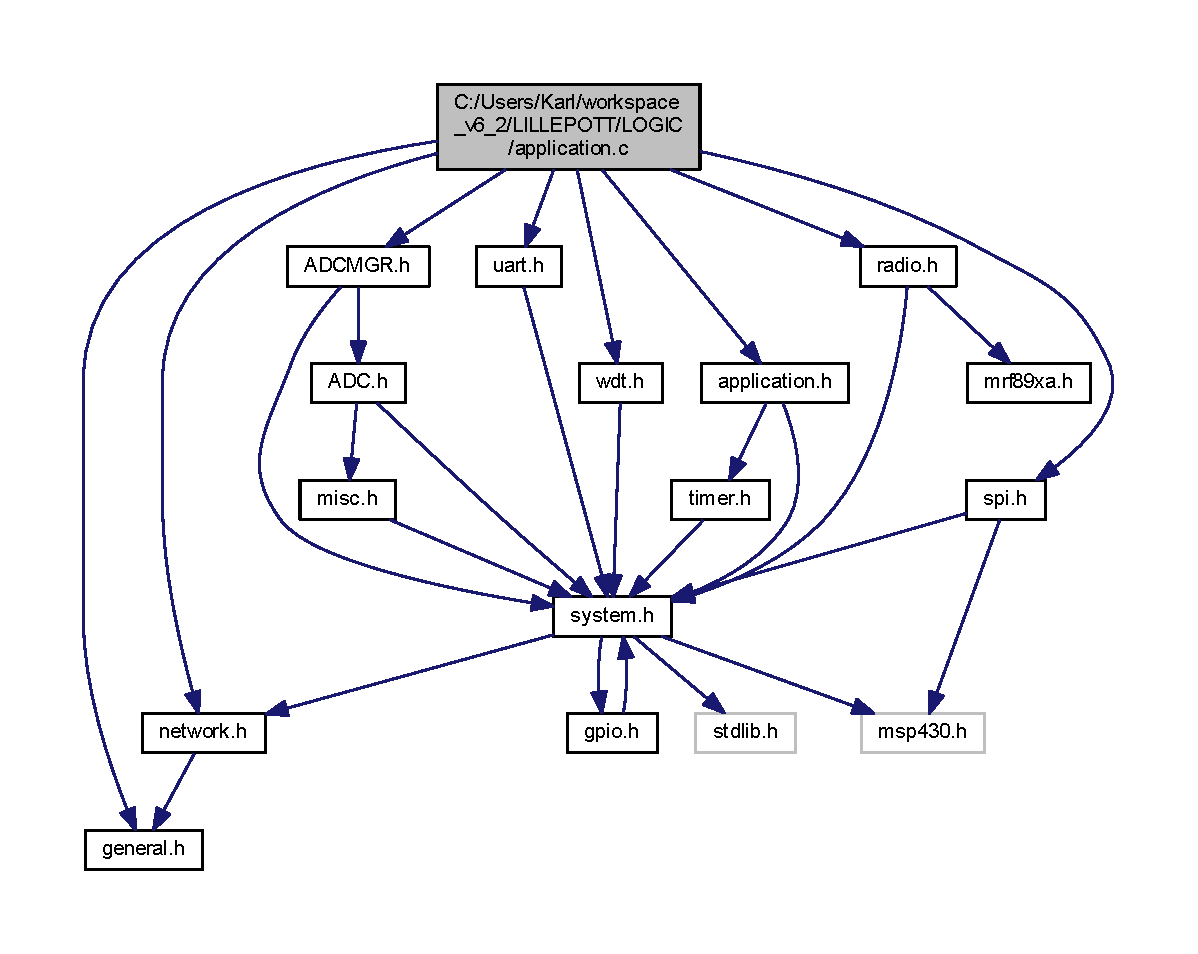
\includegraphics[width=350pt]{application_8c__incl}
\end{center}
\end{figure}
\subsection*{Typedefs}
\begin{DoxyCompactItemize}
\item 
\mbox{\Hypertarget{application_8c_a0ff87ae1f571df4aff2994259eacaebf}\label{application_8c_a0ff87ae1f571df4aff2994259eacaebf}} 
typedef enum A\+P\+P\+\_\+\+State {\bfseries A\+P\+P\+\_\+\+State}
\end{DoxyCompactItemize}
\subsection*{Enumerations}
\begin{DoxyCompactItemize}
\item 
\mbox{\Hypertarget{application_8c_ae6826746c710462d27cb1a26b914d02b}\label{application_8c_ae6826746c710462d27cb1a26b914d02b}} 
enum {\bfseries A\+P\+P\+\_\+\+State} \{ \newline
{\bfseries S\+L\+E\+EP} = 0, 
{\bfseries I\+N\+IT} = 1, 
{\bfseries T\+R\+A\+N\+S\+M\+IT} = 2, 
{\bfseries R\+E\+C\+E\+I\+VE} = 3, 
\newline
{\bfseries A\+P\+P\+\_\+\+M\+E\+A\+S\+U\+R\+E\+\_\+\+T\+E\+MP} = 4, 
{\bfseries A\+P\+P\+\_\+\+M\+E\+A\+S\+U\+R\+E\+\_\+\+H\+UM} = 5, 
{\bfseries A\+P\+P\+\_\+\+M\+E\+A\+S\+U\+R\+E\+\_\+\+B\+A\+T\+T\+E\+RY} = 6, 
{\bfseries A\+D\+J\+U\+S\+T\+\_\+\+R\+F\+\_\+\+P\+O\+W\+ER} = 7, 
\newline
{\bfseries P\+R\+E\+P\+A\+R\+E\+\_\+\+T\+O\+\_\+\+S\+L\+E\+EP} = 8, 
{\bfseries P\+A\+R\+S\+E\+\_\+\+H\+E\+A\+D\+E\+RS} = 9, 
{\bfseries N\+U\+M\+B\+E\+R\+\_\+\+O\+F\+\_\+\+A\+P\+P\+\_\+\+S\+T\+A\+T\+ES}
 \}
\end{DoxyCompactItemize}
\subsection*{Functions}
\begin{DoxyCompactItemize}
\item 
\mbox{\Hypertarget{application_8c_a97257889b1e4f85d786e713badeee5e7}\label{application_8c_a97257889b1e4f85d786e713badeee5e7}} 
void {\bfseries A\+P\+P\+\_\+cyclic} ()
\end{DoxyCompactItemize}


\subsection{Detailed Description}

\begin{DoxyImageNoCaption}
  \mbox{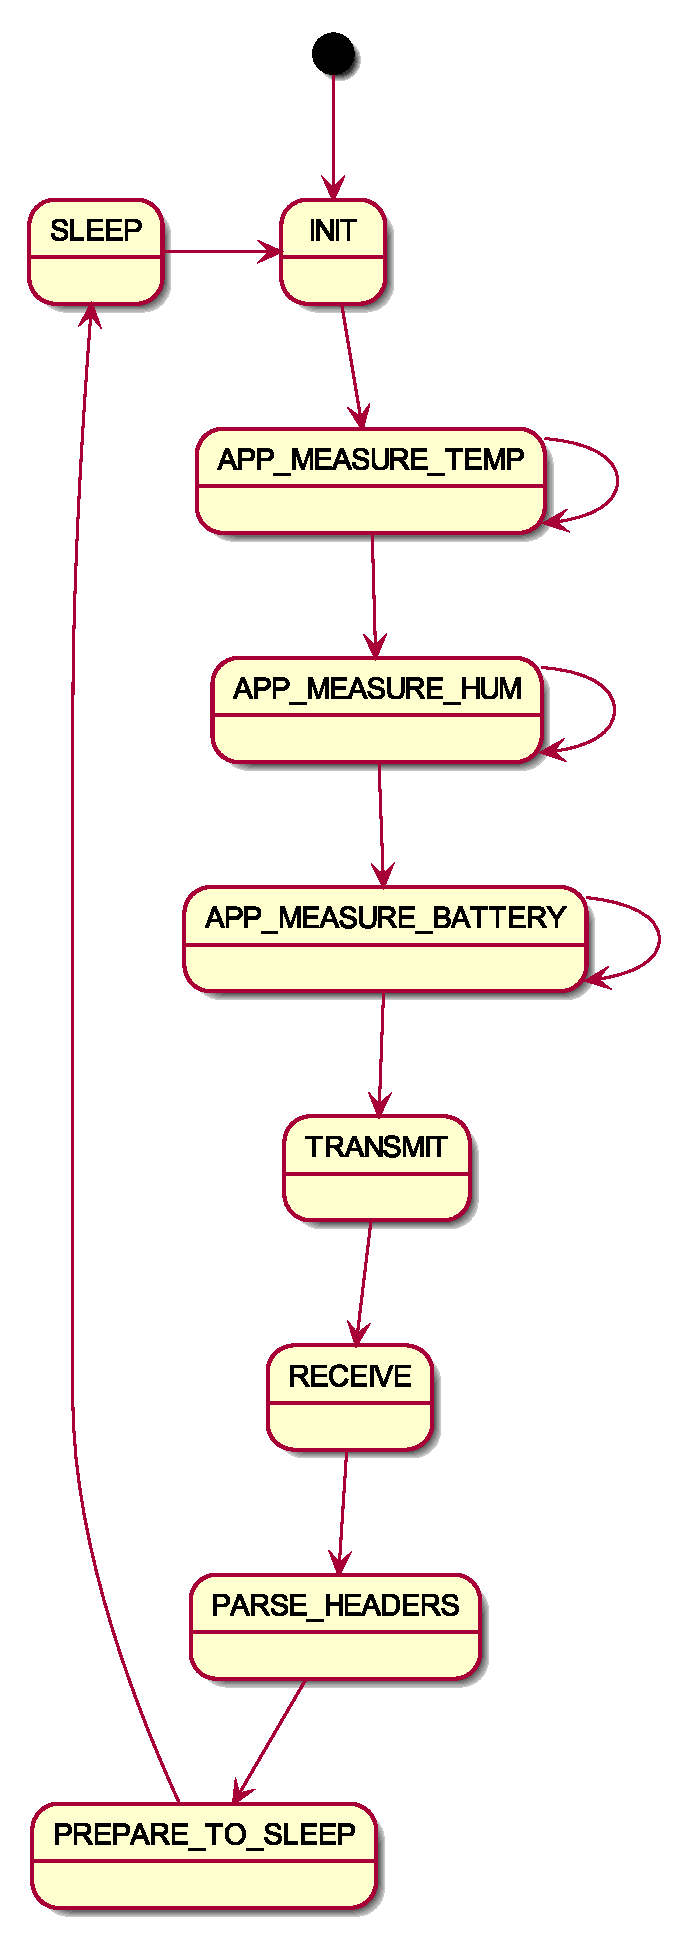
\includegraphics[width=\textwidth,height=\textheight/2,keepaspectratio=true]{APP}}
\end{DoxyImageNoCaption}
 
\hypertarget{_a_d_c_8c}{}\section{C\+:/\+Users/\+Karl/workspace\+\_\+v6\+\_\+2/\+L\+I\+L\+L\+E\+P\+O\+T\+T/\+M\+C\+U/\+A\+DC.c File Reference}
\label{_a_d_c_8c}\index{C\+:/\+Users/\+Karl/workspace\+\_\+v6\+\_\+2/\+L\+I\+L\+L\+E\+P\+O\+T\+T/\+M\+C\+U/\+A\+D\+C.\+c@{C\+:/\+Users/\+Karl/workspace\+\_\+v6\+\_\+2/\+L\+I\+L\+L\+E\+P\+O\+T\+T/\+M\+C\+U/\+A\+D\+C.\+c}}


A\+DC hardware abstraction.  


{\ttfamily \#include \char`\"{}A\+D\+C.\+h\char`\"{}}\newline
Include dependency graph for A\+D\+C.\+c\+:\nopagebreak
\begin{figure}[H]
\begin{center}
\leavevmode
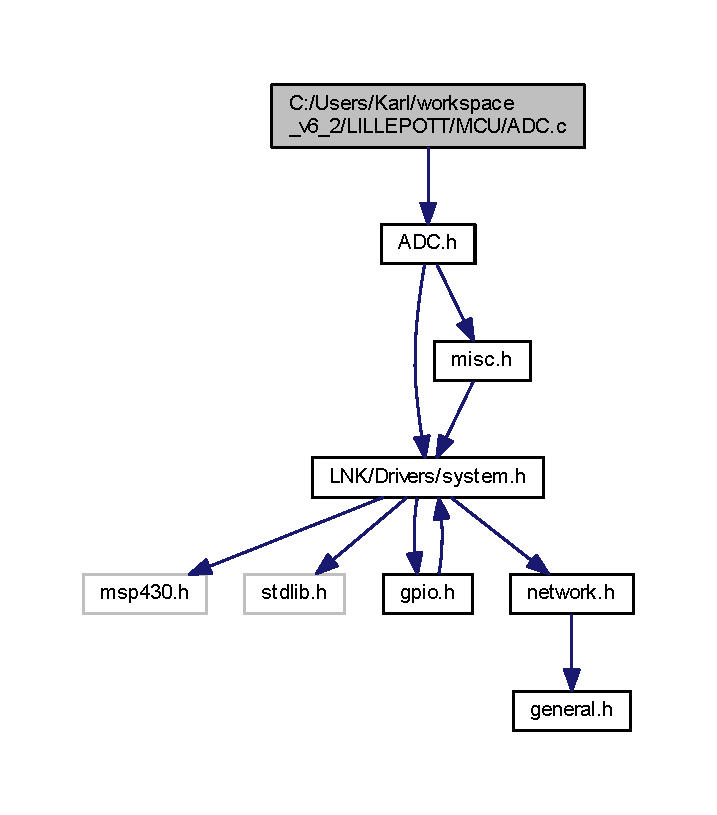
\includegraphics[width=344pt]{_a_d_c_8c__incl}
\end{center}
\end{figure}
\subsection*{Functions}
\begin{DoxyCompactItemize}
\item 
uint8 \hyperlink{_a_d_c_8c_a1cb234b7ea51d295e64b1a404b86c516}{start\+Conversion} ()
\item 
uint8 \hyperlink{_a_d_c_8c_ae93705b0a5ab89f5186f70a692b2a8c2}{check\+If\+A\+D\+C\+ON} ()
\item 
uint8 \hyperlink{_a_d_c_8c_acfcbdf5182467d938b7835ce90a351b5}{A\+D\+C\+\_\+configure\+A\+DC} (A\+D\+C\+\_\+\+Conf\+Type configuration)
\item 
\mbox{\Hypertarget{_a_d_c_8c_a2723c81d42c23dec4015a3fd529e883a}\label{_a_d_c_8c_a2723c81d42c23dec4015a3fd529e883a}} 
uint8 {\bfseries check\+If\+A\+D\+C\+Busy} ()
\item 
uint16 \hyperlink{_a_d_c_8c_ae2951f8ad65e5e5e525bb7a04d820bdd}{A\+D\+C\+\_\+measure} ()
\end{DoxyCompactItemize}


\subsection{Detailed Description}
A\+DC hardware abstraction. 



\subsection{Function Documentation}
\mbox{\Hypertarget{_a_d_c_8c_acfcbdf5182467d938b7835ce90a351b5}\label{_a_d_c_8c_acfcbdf5182467d938b7835ce90a351b5}} 
\index{A\+D\+C.\+c@{A\+D\+C.\+c}!A\+D\+C\+\_\+configure\+A\+DC@{A\+D\+C\+\_\+configure\+A\+DC}}
\index{A\+D\+C\+\_\+configure\+A\+DC@{A\+D\+C\+\_\+configure\+A\+DC}!A\+D\+C.\+c@{A\+D\+C.\+c}}
\subsubsection{\texorpdfstring{A\+D\+C\+\_\+configure\+A\+D\+C()}{ADC\_configureADC()}}
{\footnotesize\ttfamily uint8 A\+D\+C\+\_\+configure\+A\+DC (\begin{DoxyParamCaption}\item[{A\+D\+C\+\_\+\+Conf\+Type}]{configuration }\end{DoxyParamCaption})}



 Configures A\+DC registers and turns on the A\+DC returns error if refrence not settled, or invalid config, success otherwise 
\begin{DoxyImageNoCaption}
  \mbox{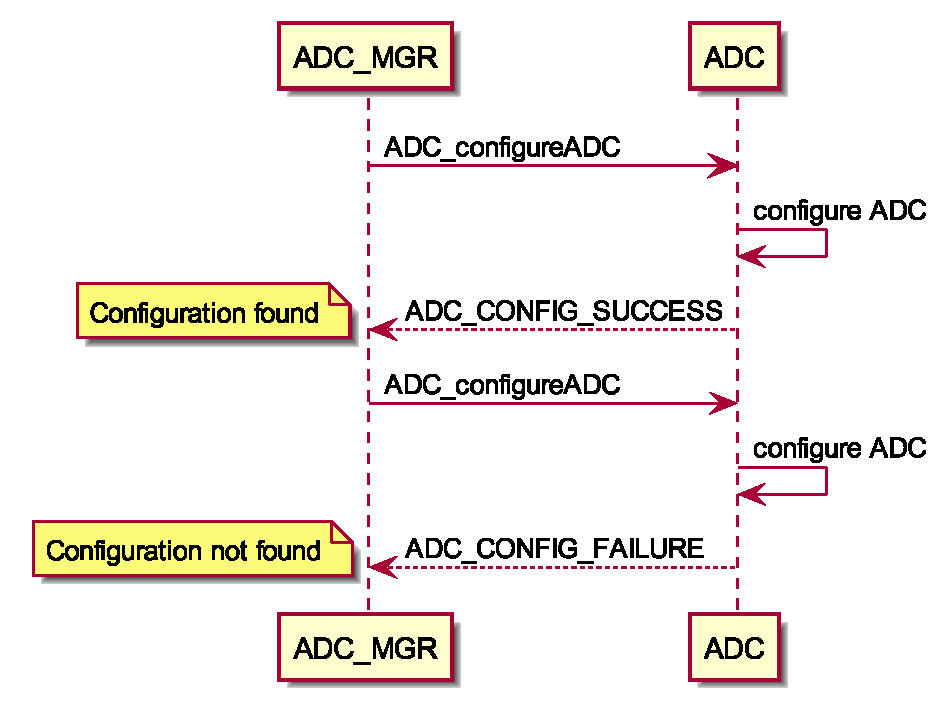
\includegraphics[width=\textwidth,height=\textheight/2,keepaspectratio=true]{ADC_configureADC}}
\end{DoxyImageNoCaption}
 \mbox{\Hypertarget{_a_d_c_8c_ae2951f8ad65e5e5e525bb7a04d820bdd}\label{_a_d_c_8c_ae2951f8ad65e5e5e525bb7a04d820bdd}} 
\index{A\+D\+C.\+c@{A\+D\+C.\+c}!A\+D\+C\+\_\+measure@{A\+D\+C\+\_\+measure}}
\index{A\+D\+C\+\_\+measure@{A\+D\+C\+\_\+measure}!A\+D\+C.\+c@{A\+D\+C.\+c}}
\subsubsection{\texorpdfstring{A\+D\+C\+\_\+measure()}{ADC\_measure()}}
{\footnotesize\ttfamily uint16 A\+D\+C\+\_\+measure (\begin{DoxyParamCaption}{ }\end{DoxyParamCaption})}



 Measures synchronously, usual call made by A\+D\+C\+M\+GR 
\begin{DoxyImageNoCaption}
  \mbox{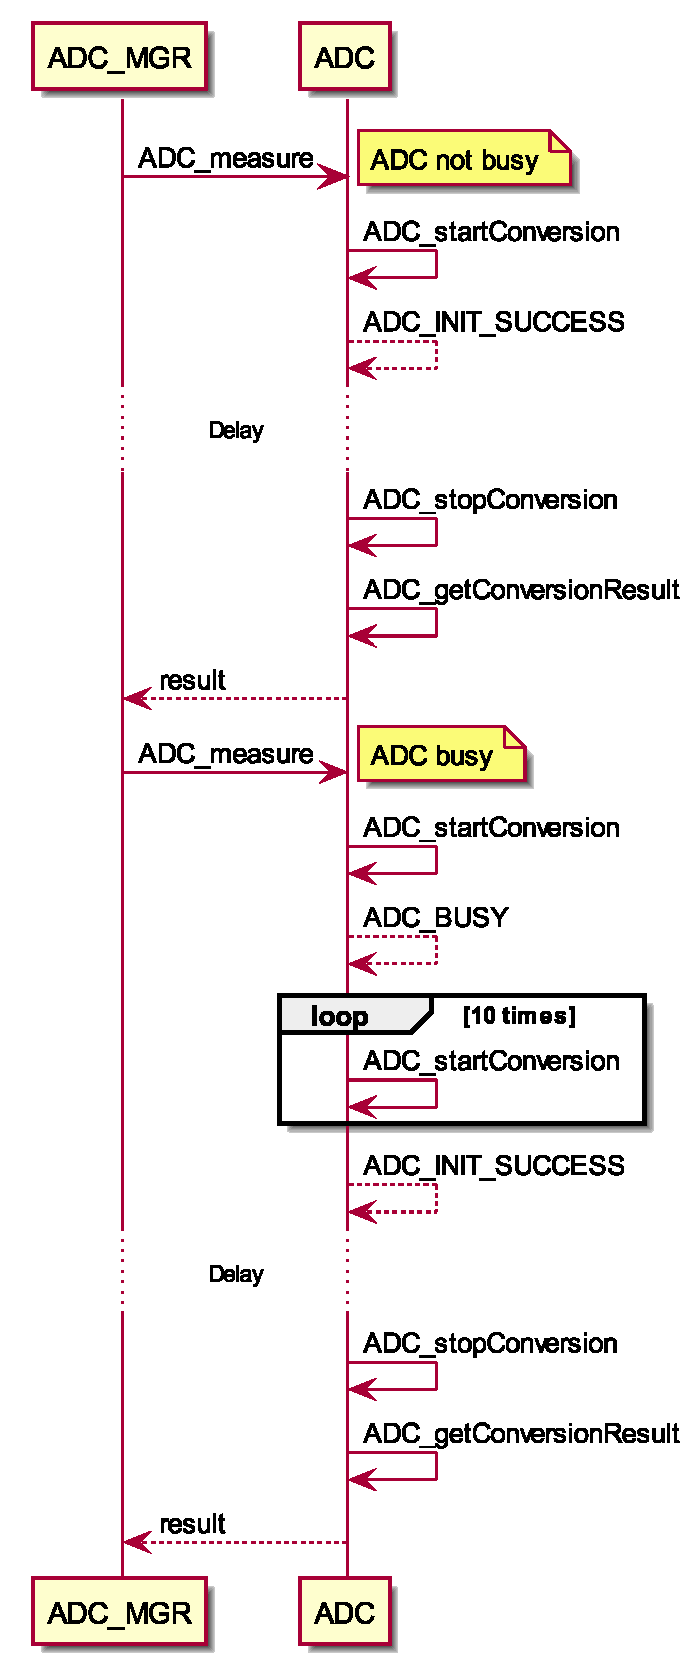
\includegraphics[width=\textwidth,height=\textheight/2,keepaspectratio=true]{ADC_MEASURE}}
\end{DoxyImageNoCaption}
 Further calibration is needed based on A\+DC configuration Does a single measurement based on configuration \begin{DoxyReturn}{Returns}
uncalibrated A\+DC conversion result (range\+: 0 to 1023) 

A\+D\+C\+\_\+\+I\+N\+V\+A\+L\+I\+D\+\_\+\+C\+O\+N\+V\+E\+R\+S\+I\+O\+N\+\_\+\+R\+E\+S\+U\+LT if A\+DC busy or it could not be configured 
\end{DoxyReturn}
Here is the call graph for this function\+:\nopagebreak
\begin{figure}[H]
\begin{center}
\leavevmode
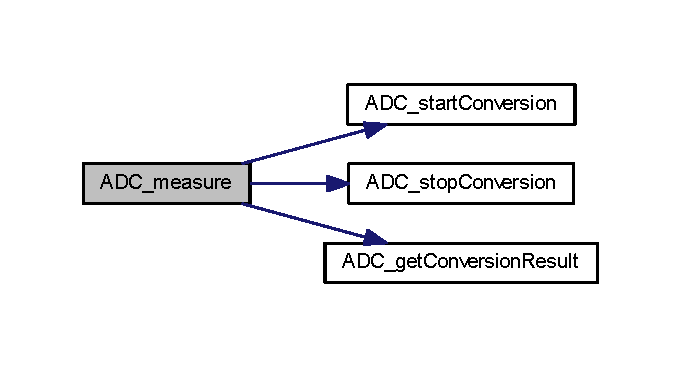
\includegraphics[width=279pt]{_a_d_c_8c_ae2951f8ad65e5e5e525bb7a04d820bdd_cgraph}
\end{center}
\end{figure}
\mbox{\Hypertarget{_a_d_c_8c_ae93705b0a5ab89f5186f70a692b2a8c2}\label{_a_d_c_8c_ae93705b0a5ab89f5186f70a692b2a8c2}} 
\index{A\+D\+C.\+c@{A\+D\+C.\+c}!check\+If\+A\+D\+C\+ON@{check\+If\+A\+D\+C\+ON}}
\index{check\+If\+A\+D\+C\+ON@{check\+If\+A\+D\+C\+ON}!A\+D\+C.\+c@{A\+D\+C.\+c}}
\subsubsection{\texorpdfstring{check\+If\+A\+D\+C\+O\+N()}{checkIfADCON()}}
{\footnotesize\ttfamily uint8 check\+If\+A\+D\+C\+ON (\begin{DoxyParamCaption}{ }\end{DoxyParamCaption})}





Check if A\+DC core is turned on Called by A\+D\+C\+\_\+configure\+A\+DC (yet to be implemented) \begin{DoxyReturn}{Returns}
1 if on, 0 otherwise 
\end{DoxyReturn}
Here is the call graph for this function\+:\nopagebreak
\begin{figure}[H]
\begin{center}
\leavevmode
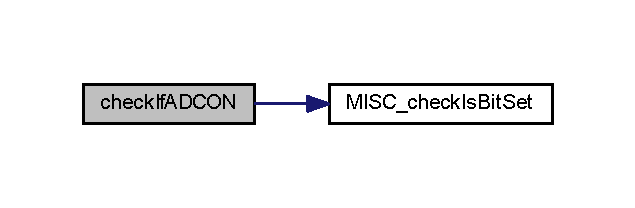
\includegraphics[width=305pt]{_a_d_c_8c_ae93705b0a5ab89f5186f70a692b2a8c2_cgraph}
\end{center}
\end{figure}
\mbox{\Hypertarget{_a_d_c_8c_a1cb234b7ea51d295e64b1a404b86c516}\label{_a_d_c_8c_a1cb234b7ea51d295e64b1a404b86c516}} 
\index{A\+D\+C.\+c@{A\+D\+C.\+c}!start\+Conversion@{start\+Conversion}}
\index{start\+Conversion@{start\+Conversion}!A\+D\+C.\+c@{A\+D\+C.\+c}}
\subsubsection{\texorpdfstring{start\+Conversion()}{startConversion()}}
{\footnotesize\ttfamily uint8 start\+Conversion (\begin{DoxyParamCaption}{ }\end{DoxyParamCaption})}



 Enables conversion and starts it if A\+D\+C10 is not busy Usually called by A\+D\+C\+\_\+measure 
\begin{DoxyImageNoCaption}
  \mbox{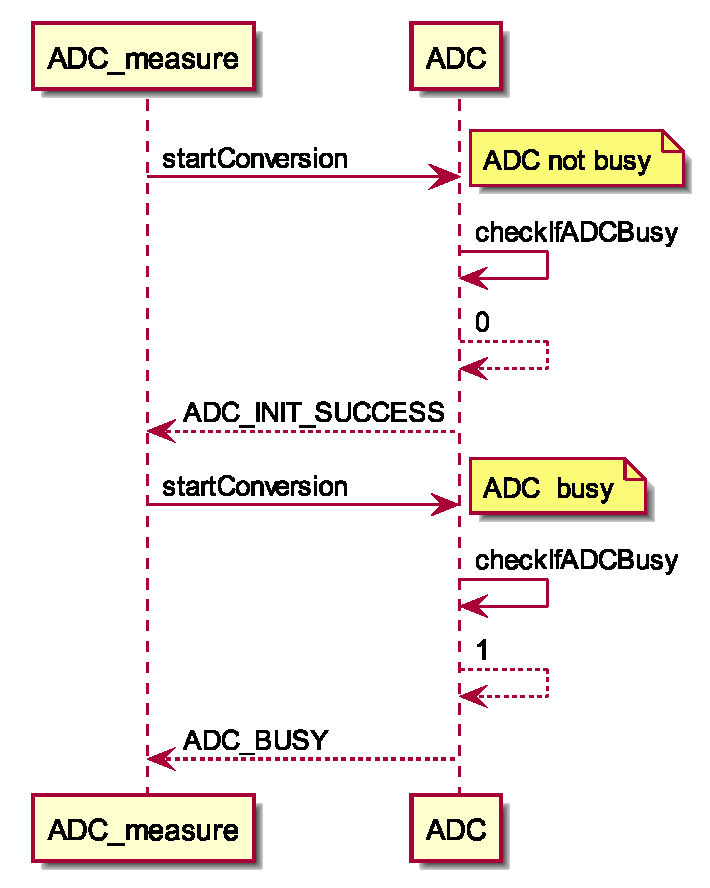
\includegraphics[width=\textwidth,height=\textheight/2,keepaspectratio=true]{startConversion}}
\end{DoxyImageNoCaption}
 \begin{DoxyReturn}{Returns}

\end{DoxyReturn}
Here is the caller graph for this function\+:\nopagebreak
\begin{figure}[H]
\begin{center}
\leavevmode
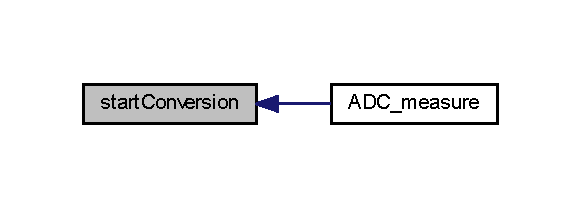
\includegraphics[width=279pt]{_a_d_c_8c_a1cb234b7ea51d295e64b1a404b86c516_icgraph}
\end{center}
\end{figure}

\hypertarget{clock_8c}{}\section{C\+:/\+Users/\+Karl/workspace\+\_\+v6\+\_\+2/\+L\+I\+L\+L\+E\+P\+O\+T\+T/\+M\+C\+U/clock.c File Reference}
\label{clock_8c}\index{C\+:/\+Users/\+Karl/workspace\+\_\+v6\+\_\+2/\+L\+I\+L\+L\+E\+P\+O\+T\+T/\+M\+C\+U/clock.\+c@{C\+:/\+Users/\+Karl/workspace\+\_\+v6\+\_\+2/\+L\+I\+L\+L\+E\+P\+O\+T\+T/\+M\+C\+U/clock.\+c}}
{\ttfamily \#include \char`\"{}clock.\+h\char`\"{}}\newline
Include dependency graph for clock.\+c\+:\nopagebreak
\begin{figure}[H]
\begin{center}
\leavevmode
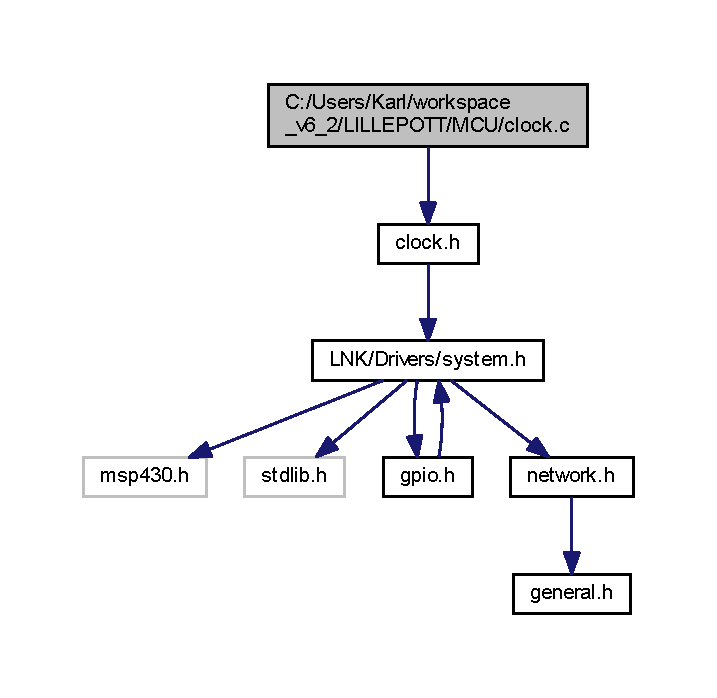
\includegraphics[width=344pt]{clock_8c__incl}
\end{center}
\end{figure}
\subsection*{Functions}
\begin{DoxyCompactItemize}
\item 
void \hyperlink{clock_8c_a614c5ac4ac1165e073ce4b6e261c2dcf}{C\+L\+K\+\_\+init\+Clk} ()
\end{DoxyCompactItemize}


\subsection{Function Documentation}
\mbox{\Hypertarget{clock_8c_a614c5ac4ac1165e073ce4b6e261c2dcf}\label{clock_8c_a614c5ac4ac1165e073ce4b6e261c2dcf}} 
\index{clock.\+c@{clock.\+c}!C\+L\+K\+\_\+init\+Clk@{C\+L\+K\+\_\+init\+Clk}}
\index{C\+L\+K\+\_\+init\+Clk@{C\+L\+K\+\_\+init\+Clk}!clock.\+c@{clock.\+c}}
\subsubsection{\texorpdfstring{C\+L\+K\+\_\+init\+Clk()}{CLK\_initClk()}}
{\footnotesize\ttfamily void C\+L\+K\+\_\+init\+Clk (\begin{DoxyParamCaption}{ }\end{DoxyParamCaption})}


\begin{DoxyItemize}
\item Basic clock initialization Configures A\+C\+LK for watchdog module, other clocks init in M\+R\+F\+\_\+\+L\+NK System\+\_\+\+Init function 
\end{DoxyItemize}
\hypertarget{misc_8c}{}\section{C\+:/\+Users/\+Karl/workspace\+\_\+v6\+\_\+2/\+L\+I\+L\+L\+E\+P\+O\+T\+T/\+M\+C\+U/misc.c File Reference}
\label{misc_8c}\index{C\+:/\+Users/\+Karl/workspace\+\_\+v6\+\_\+2/\+L\+I\+L\+L\+E\+P\+O\+T\+T/\+M\+C\+U/misc.\+c@{C\+:/\+Users/\+Karl/workspace\+\_\+v6\+\_\+2/\+L\+I\+L\+L\+E\+P\+O\+T\+T/\+M\+C\+U/misc.\+c}}
{\ttfamily \#include \char`\"{}misc.\+h\char`\"{}}\newline
Include dependency graph for misc.\+c\+:\nopagebreak
\begin{figure}[H]
\begin{center}
\leavevmode
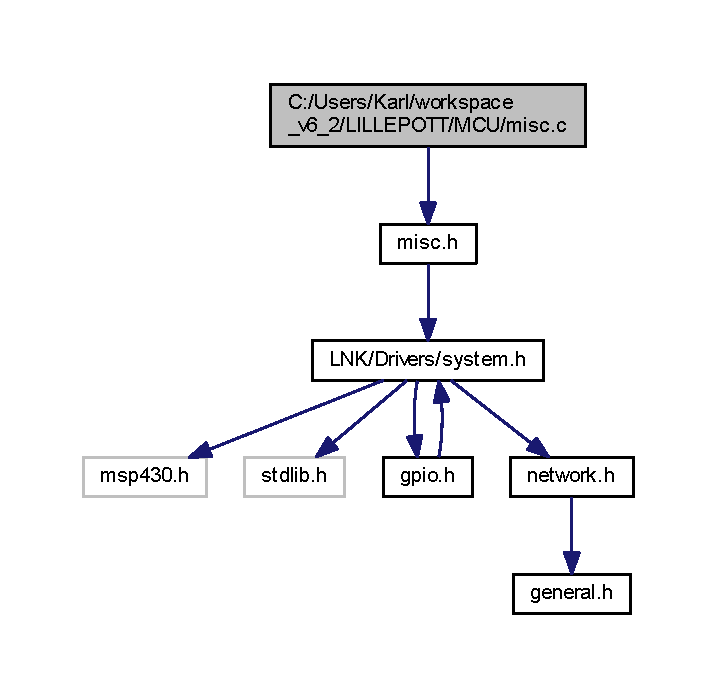
\includegraphics[width=344pt]{misc_8c__incl}
\end{center}
\end{figure}
\subsection*{Functions}
\begin{DoxyCompactItemize}
\item 
uint8 \hyperlink{misc_8c_a98a2b3c213168f5da4220764b6cf6e4d}{M\+I\+S\+C\+\_\+check\+Is\+Bit\+Set} (uint16 registerr, uint16 position)
\end{DoxyCompactItemize}


\subsection{Function Documentation}
\mbox{\Hypertarget{misc_8c_a98a2b3c213168f5da4220764b6cf6e4d}\label{misc_8c_a98a2b3c213168f5da4220764b6cf6e4d}} 
\index{misc.\+c@{misc.\+c}!M\+I\+S\+C\+\_\+check\+Is\+Bit\+Set@{M\+I\+S\+C\+\_\+check\+Is\+Bit\+Set}}
\index{M\+I\+S\+C\+\_\+check\+Is\+Bit\+Set@{M\+I\+S\+C\+\_\+check\+Is\+Bit\+Set}!misc.\+c@{misc.\+c}}
\subsubsection{\texorpdfstring{M\+I\+S\+C\+\_\+check\+Is\+Bit\+Set()}{MISC\_checkIsBitSet()}}
{\footnotesize\ttfamily uint8 M\+I\+S\+C\+\_\+check\+Is\+Bit\+Set (\begin{DoxyParamCaption}\item[{uint16}]{registerr,  }\item[{uint16}]{position }\end{DoxyParamCaption})}



 int position -\/ position of the bit to be checked L\+SB is 0th bit Returns 1 if the bit is set

\begin{DoxyReturn}{Returns}
1 when set, 0 otherwise 
\end{DoxyReturn}

\begin{DoxyParams}{Parameters}
{\em registerr} & System register to be checked \\
\hline
{\em position} & bit to be checked, L\+SB is 0th bit \\
\hline
\end{DoxyParams}
Here is the caller graph for this function\+:\nopagebreak
\begin{figure}[H]
\begin{center}
\leavevmode
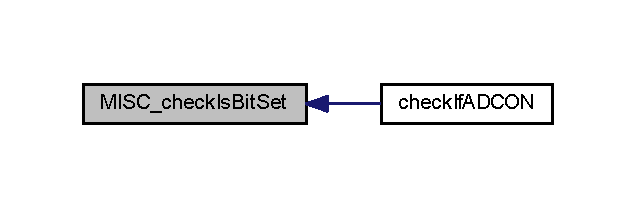
\includegraphics[width=305pt]{misc_8c_a98a2b3c213168f5da4220764b6cf6e4d_icgraph}
\end{center}
\end{figure}

\hypertarget{wdt_8c}{}\section{C\+:/\+Users/\+Karl/workspace\+\_\+v6\+\_\+2/\+L\+I\+L\+L\+E\+P\+O\+T\+T/\+M\+C\+U/wdt.c File Reference}
\label{wdt_8c}\index{C\+:/\+Users/\+Karl/workspace\+\_\+v6\+\_\+2/\+L\+I\+L\+L\+E\+P\+O\+T\+T/\+M\+C\+U/wdt.\+c@{C\+:/\+Users/\+Karl/workspace\+\_\+v6\+\_\+2/\+L\+I\+L\+L\+E\+P\+O\+T\+T/\+M\+C\+U/wdt.\+c}}


Documentation for the watchdog module.  


{\ttfamily \#include $<$wdt.\+h$>$}\newline
Include dependency graph for wdt.\+c\+:
\nopagebreak
\begin{figure}[H]
\begin{center}
\leavevmode
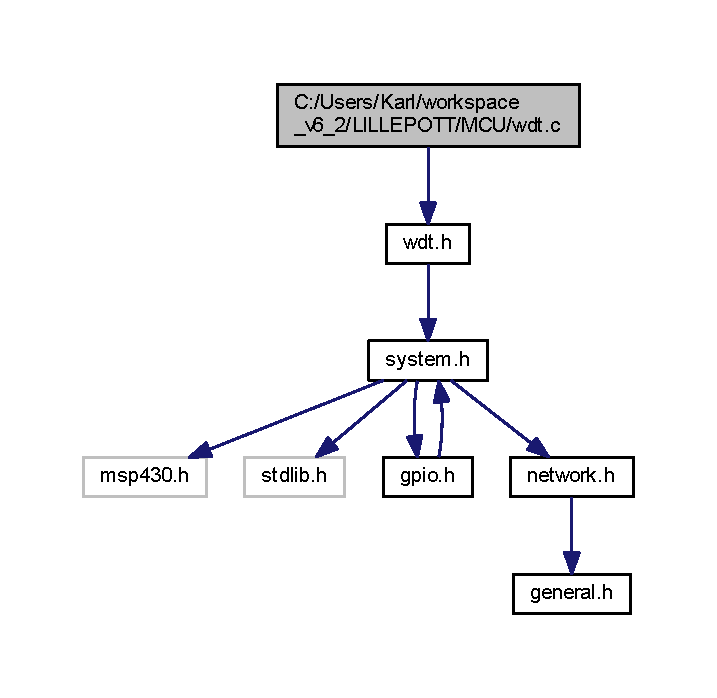
\includegraphics[width=344pt]{wdt_8c__incl}
\end{center}
\end{figure}
\subsection*{Functions}
\begin{DoxyCompactItemize}
\item 
void \hyperlink{wdt_8c_a3326de6d0c209742242f25167d0894fb}{W\+D\+T\+\_\+configure} ()
\item 
uint32 \hyperlink{wdt_8c_a1ec95cdd432b1667b6d2ead9802ab869}{W\+D\+T\+\_\+get\+Current\+Period} ()
\item 
uint8 \hyperlink{wdt_8c_a1ca55bccb8a02d85f97804444f99afa0}{W\+D\+T\+\_\+set\+Watchdog} (uint32 period)
\item 
\mbox{\Hypertarget{wdt_8c_ac6e80bdf33b7d96bf2ed52ecbf08423a}\label{wdt_8c_ac6e80bdf33b7d96bf2ed52ecbf08423a}} 
\+\_\+\+\_\+interrupt void {\bfseries watchdog\+\_\+timer} (void)
\end{DoxyCompactItemize}
\subsection*{Variables}
\begin{DoxyCompactItemize}
\item 
uint32 \hyperlink{wdt_8c_a3312a478f58f673bdeb781a8f34b3249}{wdt\+Counter} = 0
\item 
uint32 \hyperlink{wdt_8c_acd668f83c1bcd64c726a03065168278a}{wdt\+Current\+Period} = 0
\item 
\mbox{\Hypertarget{wdt_8c_a8f839d32a9c0153fd998d475eaffee92}\label{wdt_8c_a8f839d32a9c0153fd998d475eaffee92}} 
uint16 {\bfseries f\+Measurement}
\end{DoxyCompactItemize}


\subsection{Detailed Description}
Documentation for the watchdog module. 



\subsection{Function Documentation}
\mbox{\Hypertarget{wdt_8c_a3326de6d0c209742242f25167d0894fb}\label{wdt_8c_a3326de6d0c209742242f25167d0894fb}} 
\index{wdt.\+c@{wdt.\+c}!W\+D\+T\+\_\+configure@{W\+D\+T\+\_\+configure}}
\index{W\+D\+T\+\_\+configure@{W\+D\+T\+\_\+configure}!wdt.\+c@{wdt.\+c}}
\subsubsection{\texorpdfstring{W\+D\+T\+\_\+configure()}{WDT\_configure()}}
{\footnotesize\ttfamily void W\+D\+T\+\_\+configure (\begin{DoxyParamCaption}{ }\end{DoxyParamCaption})}



 Configures watchdog module Here is the caller graph for this function\+:
\nopagebreak
\begin{figure}[H]
\begin{center}
\leavevmode
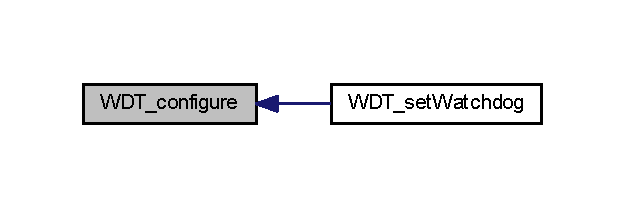
\includegraphics[width=300pt]{wdt_8c_a3326de6d0c209742242f25167d0894fb_icgraph}
\end{center}
\end{figure}
\mbox{\Hypertarget{wdt_8c_a1ec95cdd432b1667b6d2ead9802ab869}\label{wdt_8c_a1ec95cdd432b1667b6d2ead9802ab869}} 
\index{wdt.\+c@{wdt.\+c}!W\+D\+T\+\_\+get\+Current\+Period@{W\+D\+T\+\_\+get\+Current\+Period}}
\index{W\+D\+T\+\_\+get\+Current\+Period@{W\+D\+T\+\_\+get\+Current\+Period}!wdt.\+c@{wdt.\+c}}
\subsubsection{\texorpdfstring{W\+D\+T\+\_\+get\+Current\+Period()}{WDT\_getCurrentPeriod()}}
{\footnotesize\ttfamily uint32 W\+D\+T\+\_\+get\+Current\+Period (\begin{DoxyParamCaption}{ }\end{DoxyParamCaption})}



 interface for getting current set W\+DT period count \begin{DoxyReturn}{Returns}
wdt\+Current\+Period 
\end{DoxyReturn}
\mbox{\Hypertarget{wdt_8c_a1ca55bccb8a02d85f97804444f99afa0}\label{wdt_8c_a1ca55bccb8a02d85f97804444f99afa0}} 
\index{wdt.\+c@{wdt.\+c}!W\+D\+T\+\_\+set\+Watchdog@{W\+D\+T\+\_\+set\+Watchdog}}
\index{W\+D\+T\+\_\+set\+Watchdog@{W\+D\+T\+\_\+set\+Watchdog}!wdt.\+c@{wdt.\+c}}
\subsubsection{\texorpdfstring{W\+D\+T\+\_\+set\+Watchdog()}{WDT\_setWatchdog()}}
{\footnotesize\ttfamily uint8 W\+D\+T\+\_\+set\+Watchdog (\begin{DoxyParamCaption}\item[{uint32}]{period }\end{DoxyParamCaption})}



 Configures watchdog timer wakeup period Uses V\+LO as a source clock, which ranges from 4k\+Hz -\/ 20 k\+Hz

Acceptable input\+: 2 -\/ 31536000 (typically 7.\+2 seconds -\/ 1314 days)

minimal 2 periods (typically 2 $\ast$ 3.\+6 seconds)

typical 3.\+6 seconds per period (atleast 15 periods)

4k\+Hz = 8 second period 8k\+Hz = 4 second period 12k\+Hz = 2.\+66666 second period 20k\+Hz = 1.\+66666 second period

\begin{DoxyReturn}{Returns}
W\+D\+T\+\_\+\+S\+U\+C\+C\+E\+SS 

W\+D\+T\+\_\+\+E\+RR 
\end{DoxyReturn}

\begin{DoxyParams}{Parameters}
{\em period} & Period for watchdog, valid range\+: 2 -\/ 31536000 \\
\hline
\end{DoxyParams}
Here is the call graph for this function\+:
\nopagebreak
\begin{figure}[H]
\begin{center}
\leavevmode
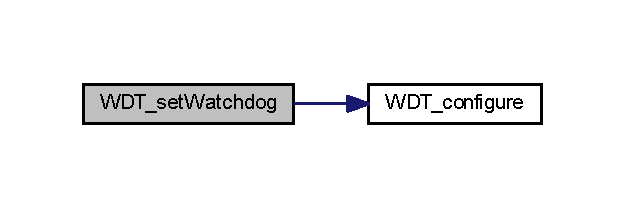
\includegraphics[width=300pt]{wdt_8c_a1ca55bccb8a02d85f97804444f99afa0_cgraph}
\end{center}
\end{figure}


\subsection{Variable Documentation}
\mbox{\Hypertarget{wdt_8c_a3312a478f58f673bdeb781a8f34b3249}\label{wdt_8c_a3312a478f58f673bdeb781a8f34b3249}} 
\index{wdt.\+c@{wdt.\+c}!wdt\+Counter@{wdt\+Counter}}
\index{wdt\+Counter@{wdt\+Counter}!wdt.\+c@{wdt.\+c}}
\subsubsection{\texorpdfstring{wdt\+Counter}{wdtCounter}}
{\footnotesize\ttfamily uint32 wdt\+Counter = 0}

Period counter, period length depends on W\+DT configuration \mbox{\Hypertarget{wdt_8c_acd668f83c1bcd64c726a03065168278a}\label{wdt_8c_acd668f83c1bcd64c726a03065168278a}} 
\index{wdt.\+c@{wdt.\+c}!wdt\+Current\+Period@{wdt\+Current\+Period}}
\index{wdt\+Current\+Period@{wdt\+Current\+Period}!wdt.\+c@{wdt.\+c}}
\subsubsection{\texorpdfstring{wdt\+Current\+Period}{wdtCurrentPeriod}}
{\footnotesize\ttfamily uint32 wdt\+Current\+Period = 0}

current configured period, default is 0, ranges from 2 to 31536000 
%--- End generated contents ---

% Index
\backmatter
\newpage
\phantomsection
\clearemptydoublepage
\addcontentsline{toc}{chapter}{Index}
\printindex

\end{document}
